\documentclass{standalone}

\usepackage[latin1]{inputenc}
\usepackage{amsmath}
\usepackage{amssymb}
\usepackage{amsthm}

\usepackage{tikz}
\usetikzlibrary{arrows}

%% generates a tightly fitting border around the work
%\usepackage[active,tightpage]{preview}
%\PreviewEnvironment{tikzpicture}
%\setlength\PreviewBorder{0.5mm}
%%\renewcommand\PreviewBbAdjust{-\PreviewBorder 1mm -1.15mm -0.85mm}

\usepackage{color}

%\pagestyle{empty}

\begin{document}

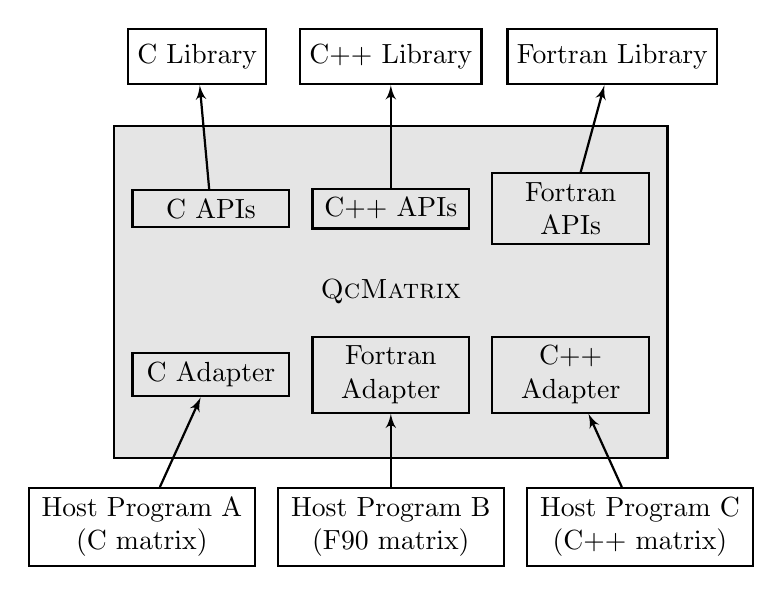
\begin{tikzpicture}[thick, node distance=85]
  \node[color=black, rectangle, draw, text badly centered, sharp corners, minimum height=120, % 
        minimum width=200, fill=black!10] (QcMatrix) {\textsc{QcMatrix}};
  % adapters
  \node[color=black, rectangle, draw, text badly centered, sharp corners, minimum height=2, %
        text width=50, xshift=-65, yshift=55, below of=QcMatrix] (CAdapter) {C Adapter};
  \node[color=black, rectangle, draw, text badly centered, sharp corners, minimum height=2, %
        text width=50, yshift=55, below of=QcMatrix] (FAdapter) {Fortran Adapter};
  \node[color=black, rectangle, draw, text badly centered, sharp corners, minimum height=2, %
        text width=50, xshift=65, yshift=55, below of=QcMatrix] (CppAdapter) {C++ Adapter};
  % APIs
  \node[color=black, rectangle, draw, text badly centered, sharp corners, minimum height=2, %
        text width=50, xshift=-65, yshift=-55, above of=QcMatrix] (CAPIs) {C APIs};
  \node[color=black, rectangle, draw, text badly centered, sharp corners, minimum height=2, %
        text width=50, yshift=-55, above of=QcMatrix] (CppAPIs) {C++ APIs};
  \node[color=black, rectangle, draw, text badly centered, sharp corners, minimum height=2, %
        text width=50, xshift=65, yshift=-55, above of=QcMatrix] (FAPIs) {Fortran APIs};
  % application libraries
  \node[color=black, rectangle, draw, text badly centered, sharp corners, minimum height=20, %
        above of=QcMatrix, xshift=-70] (LibAppC) {C Library};
  \node[color=black, rectangle, draw, text badly centered, sharp corners, minimum height=20, %
        above of=QcMatrix] (LibAppCpp) {C++ Library};
  \node[color=black, rectangle, draw, text badly centered, sharp corners, minimum height=20, %
        above of=QcMatrix, xshift=80] (LibAppF) {Fortran Library};
  % host programs
  \node[color=black, rectangle, draw, text badly centered, sharp corners, minimum height=20, %
        text width=75, below of=QcMatrix, xshift=-90] (HostProgA) {Host Program A\linebreak(C matrix)};
  \node[color=black, rectangle, draw, text badly centered, sharp corners, minimum height=20, %
        text width=75, below of=QcMatrix] (HostProgB) {Host Program B\linebreak(F90 matrix)};
  \node[color=black, rectangle, draw, text badly centered, sharp corners, minimum height=20, %
        text width=75, below of=QcMatrix, xshift=90] (HostProgC) {Host Program C\linebreak(C++ matrix)};
  \draw [color=black, -latex'] (CAPIs)--(LibAppC);
  \draw [color=black, -latex'] (CppAPIs)--(LibAppCpp);
  \draw [color=black, -latex'] (FAPIs)--(LibAppF);
  \draw [color=black, -latex'] (HostProgA)--(CAdapter);
  \draw [color=black, -latex'] (HostProgB)--(FAdapter);
  \draw [color=black, -latex'] (HostProgC)--(CppAdapter);
\end{tikzpicture}

\end{document}
